\documentclass[10pt, aspectratio=169]{beamer}

% Pacotes essenciais
\usepackage[utf8]{inputenc}
\usepackage[T1]{fontenc}
\usepackage[portuguese]{babel}
\usepackage{booktabs}
\usepackage{fontawesome5}
\usepackage{graphicx}
\usepackage{multicol}

% Tema e cores
\usetheme{Madrid}
\usecolortheme{default}

% Configurações de título
\title[Semantic Movie Search]{Semantic Movie Search}
\subtitle{Busca semântica de filmes em linguagem natural, com resposta formatada por um LLM local}
\author[PAA - UnB]{PROJETO E ANÁLISE DE ALGORITMOS }
\institute[UnB]{Universidade de Brasília (UnB) \\ 2026.1}
\date{06/07/2026}

\begin{document}

% ---------------------------------------------------
% Slide 1: Título
% ---------------------------------------------------
\begin{frame}
    \titlepage
\end{frame}

% ---------------------------------------------------
% Slide 2: Roteiro da apresentação
% ---------------------------------------------------
\begin{frame}{Roteiro da apresentação}
    \vspace{0.5cm}
    \begin{columns}[T]
        \begin{column}{0.5\textwidth}
            \begin{enumerate}
                \item Integrantes do grupo
                \item Linguagens, bibliotecas e licenças
                \item Programas: servidor, banco de dados
                \item Como o sistema vai funcionar
                \item Dados de treinamento (dataset)
                \item Pré-processamento e complexidade
                \item Treinamento dos modelos
            \end{enumerate}
        \end{column}
        \begin{column}{0.5\textwidth}
            \begin{enumerate}
                \setcounter{enumi}{7}
                \item Como o servidor forma a resposta
                \item Recursos computacionais disponíveis
                \item Tempo de execução de cada fase
                \item Tempo de treino x qualidade
                \item Tempo de inferência x qualidade
                \item Demais aspectos relevantes
            \end{enumerate}
        \end{column}
    \end{columns}
\end{frame}

% ---------------------------------------------------
% Slide 3: Ponto 1 - Integrantes
% ---------------------------------------------------
\begin{frame}{1. Integrantes do grupo}
    \begin{center}
        \Huge \faUsers
    \end{center}
    \vspace{0.5cm}
    \begin{itemize}
        \item \textbf{Daniel Hollenbach} - Matrícula: 241020859
        \item \textbf{Davi Bragança} - Matrícula: 242001473
        \item \textbf{Davi Galvão} - Matrícula: 241038577 
        \item \textbf{Lucas Mendes} - Matrícula: 241020750 
        \item \textbf{Pedro Marcinoni} - Matrícula: 241002396 
    \end{itemize}
    
    \vspace{0.5cm}
\end{frame}

% ---------------------------------------------------
% Slide 4: Pontos 2 e 3 - Tecnologias
% ---------------------------------------------------
\begin{frame}{2 e 3. Linguagens, bibliotecas e programas}
    \begin{itemize}
        \item \textbf{Linguagem Principal:} Python 3.11
        \vspace{0.3cm}
        \item \textbf{Bibliotecas e Licenças:} 
        \begin{itemize}
            \item \texttt{sentence-transformers}, \texttt{faiss-cpu}, \texttt{gensim}, \texttt{scikit-learn}, \texttt{streamlit}, \texttt{pandas}.
            \item Todas são \textit{open source} (licenças MIT/Apache/BSD).
        \end{itemize}
        \vspace{0.3cm}
        \item \textbf{Programas / Servidor:}
        \begin{itemize}
            \item Interface local em \textbf{Streamlit} (\texttt{streamlit run app.py}).
            \item LLM local rodando via \textbf{Ollama} (modelo Phi-4 Mini).
        \end{itemize}
        \vspace{0.3cm}
        \item \textbf{Banco de Dados:}
        \begin{itemize}
            \item Nenhum SGBD tradicional. Dados servidos a partir de arquivos \texttt{CSV} + arquivos \texttt{.npy} / \texttt{.faiss} carregados diretamente em memória (viável dado o escopo e tamanho do dataset).
        \end{itemize}
    \end{itemize}
\end{frame}

% ---------------------------------------------------
% Slide 5: Ponto 4 - Arquitetura
% ---------------------------------------------------
\begin{frame}{4. Como o sistema vai funcionar}
    \begin{center}
        \Large \faSitemap \quad Fluxo da Arquitetura
    \end{center}
    
    \vspace{0.3cm}
    \begin{enumerate}
        \item \textbf{Entrada:} Usuário digita a pergunta na interface.
        \item \textbf{Processamento da Query:} \texttt{format\_query()} processa a entrada.
        \item \textbf{Busca Semântica:} Execução de 1 dos 4 métodos de busca (escolhido pelo usuário na interface para fins de comparação).
        \item \textbf{Padronização:} Resultados formatados através da função \texttt{build\_result}.
        \item \textbf{Geração de Texto:} LLM local recebe o contexto recuperado e formata a resposta.
        \item \textbf{Saída:} Exibição do resultado final na interface do Streamlit.
    \end{enumerate}
\end{frame}

% ---------------------------------------------------
% Slide 6: Ponto 5 - Dataset (Origem)
% ---------------------------------------------------
\begin{frame}{5. Dados de treinamento (Dataset)}
    \framesubtitle{Origem, escopo e obtenção}
    
    \textbf{Dataset: CMU Movie Summary Corpus}
    \begin{itemize}
        \item Criado por Bamman, O'Connor \& Smith -- \textit{"Learning Latent Personas of Film Characters"}, ACL 2013.
        \item \textbf{Origem:}
        \begin{itemize}
            \item Sinopses extraídas do dump da Wikipédia em inglês (nov/2012).
            \item Metadados extraídos do dump do Freebase (nov/2012).
        \end{itemize}
        \item \textbf{Licença:} Creative Commons Attribution-ShareAlike.
        \item \textbf{Obtenção:} Download direto de arquivos compactados (\texttt{.tar.gz}) da página pública do grupo ARK (CMU) -- sem necessidade de \textit{scraping}.
    \end{itemize}
    
    \vspace{0.3cm}
    \begin{columns}
        \begin{column}{0.33\textwidth}
            \centering
            \Large \textbf{42.306} \\
            \normalsize sinopses de filmes
        \end{column}
        \begin{column}{0.33\textwidth}
            \centering
            \Large \textbf{81.741} \\
            \normalsize filmes c/ metadados
        \end{column}
     %   \begin{column}{0.33\textwidth}
      %      \centering
       %     \Large \textbf{450.669} \\
       %     \normalsize personagens
       % \end{column}
    \end{columns}
\end{frame}

% ---------------------------------------------------
% Slide 7: Ponto 5 - Dataset (Arquivos)
% ---------------------------------------------------
\begin{frame}{5. Dados de treinamento (Arquivos)}
    \framesubtitle{Tamanho e subconjunto de trabalho}
    
    \begin{table}[]
        \centering
        \small
        \begin{tabular}{@{}p{4cm} p{1.5cm} p{7.5cm}@{}}
            \toprule
            \textbf{Arquivo} & \textbf{Tamanho} & \textbf{Conteúdo} \\
            \midrule
            \texttt{plot\_summaries.txt} & 29 MB & Sinopses (ID Wikipédia + texto) \\
            \texttt{movie.metadata.tsv} & 3,4 MB & Título, data, receita, gêneros (Freebase) \\
          %  \texttt{character.metadata.tsv} & 14 MB & 450.669 personagens (nome, idade, gênero ator) \\
         %   \texttt{tvtropes.clusters.txt} & 58 KB & 72 tipos de persona, 501 instâncias (avaliação) \\
        %    \texttt{name.clusters.txt} & 65 KB & 970 nomes recorrentes em $>1$ filme \\
            \bottomrule
        \end{tabular}
    \end{table}
    
    \vspace{0.3cm}
    \textbf{Subconjunto utilizado:} 
    \textit{Merge} (\textit{inner join} pelo ID da Wikipédia) entre sinopses e metadados, resultando em \textbf{42.204 filmes} (sinopse + gênero). Os 4 métodos de busca operam exclusivamente sobre esse subconjunto.
\end{frame}

% ---------------------------------------------------
% Slide 8: Ponto 6 - Pré-processamento
% ---------------------------------------------------
\begin{frame}{6. Pré-processamento e complexidade}
    \framesubtitle{Pipeline de dados (\texttt{clean\_data.py})}
    
    \begin{enumerate}
        \item \textbf{Merge dos dados:} \\
        União dos arquivos por ID (\textit{inner join}). \\
        \textit{Complexidade:} $\mathcal{O}(N \log N)$
        
        \item \textbf{Parse de gêneros:} \\
        Dicionário Freebase (JSON) $\rightarrow$ string "Gênero1;Gênero2" na coluna \texttt{Genres\_clean}. \\
        \textit{Complexidade:} $\mathcal{O}(N \cdot g)$
        
        \item \textbf{Limpeza de texto:} \\
        Remoção de pontuação + \textit{lowercase} da sinopse $\rightarrow$ \texttt{Clean\_summary}. \\
        \textit{Complexidade:} $\mathcal{O}(N \cdot L)$
        
        \item \textbf{Exportação:} \\
        Geração do \texttt{processed\_movies.csv} (42.204 linhas $\times$ 6 colunas). \\
        \textit{Complexidade:} $\mathcal{O}(N)$
    \end{enumerate}
    
    \vspace{0.2cm}
    \footnotesize{\textit{* $N$ = filmes, $L$ = tamanho da sinopse, $g$ = qtd. de gêneros. O custo é dominado pela limpeza de texto, linear no volume do corpus.}}
\end{frame}

% ---------------------------------------------------
% Slide 9: Ponto 6 - Resolução de bug
% ---------------------------------------------------


% ---------------------------------------------------
% Slide 10: Ponto 7 - Treinamento
% ---------------------------------------------------
\begin{frame}{7. Treinamento dos modelos}
    \begin{itemize}
        \item \textbf{Word2Vec:} 
        \begin{itemize}
            \item Treinado do zero sobre o corpus (\texttt{gensim}).
            \item Hiperparâmetros principais: \texttt{vector\_size=100}, \texttt{window=5}, \texttt{min\_count=1}.
        \end{itemize}
        \vspace{0.3cm}
        \item \textbf{Sentence Embeddings:}
        \begin{itemize}
            \item Uso de modelo pré-treinado (\texttt{all-MiniLM-L6-v2}).
            \item Sem necessidade de \textit{fine-tuning} (diferença chave em relação à abordagem Word2Vec).
        \end{itemize}
        \vspace{0.3cm}
        \item \textbf{HNSW (FAISS):}
        \begin{itemize}
            \item Índice \texttt{IndexHNSWFlat} construído sobre os embeddings.
            \item Normalização L2 aplicada; Parâmetro $M=32$.
            \item Complexidade de indexação vs. latência de consulta sub-linear na inferência.
        \end{itemize}
    \end{itemize}
\end{frame}

% ---------------------------------------------------
% Slide 11: Ponto 8 - Formação da resposta
% ---------------------------------------------------
\begin{frame}{8. Como o servidor forma a resposta}
    \begin{itemize}
        \item \textbf{Injeção de Contexto (RAG):}
        \begin{itemize}
            \item Apenas as sinopses mais relevantes (recuperadas pelo \texttt{top\_k} da busca semântica) são passadas ao LLM.
            \item O corpus inteiro nunca é carregado no \textit{prompt}.
        \end{itemize}
        \vspace{0.3cm}
        \item \textbf{Configuração do LLM Local:}
        \begin{itemize}
            \item Modelo: Phi-4 Mini rodando no Ollama.
            \item \textit{Prompt} determinístico: \texttt{temperature=0} e \texttt{top\_p=0.1} (escolha técnica para mitigar alucinações e focar nos fatos da sinopse).
        \end{itemize}
        \vspace{0.3cm}
        \item \textbf{Latência e Resiliência:}
        \begin{itemize}
            \item A etapa de geração é o gargalo de latência, sendo dependente do tamanho do contexto enviado.
            \item Fallback implementado caso a API do Ollama fique offline.
        \end{itemize}
    \end{itemize}
\end{frame}

% ---------------------------------------------------
% Slide 12: Pontos 9 e 10 - Hardware e Tempo
% ---------------------------------------------------
\begin{frame}{9 e 10. Recursos e Tempo de Execução}
    \begin{itemize}
        \item \textbf{Recursos Computacionais Disponíveis:}
        \begin{itemize}
            \item Notebook: Intel Core i7-11800H (8c/16t), 16\,GB RAM, GPU RTX 3050 Ti --- execução em CPU (\texttt{faiss-cpu} + modelos em CPU).
            \item Justifica viabilidade do Word2Vec do zero vs. impossibilidade de \textit{fine-tuning} local de LLMs pesados.
        \end{itemize}
        \vspace{0.2cm}
        \item \textbf{Tempos Medidos por Fase:}
        \begin{itemize}
            \item \textbf{Pré-processamento:} $\sim$2s (merge + parse de gêneros + limpeza).
            \item \textbf{Geração de Embeddings (MiniLM):} $\sim$73s.
            \item \textbf{Treinamento Word2Vec:} $\sim$30s (treino + vetores-médio).
            \item \textbf{Índice HNSW:} $\sim$2s (sobre os embeddings prontos).
        \end{itemize}
        \vspace{0.2cm}
        \item \textbf{Comparativo dos 4 métodos de busca:}
        \begin{itemize}
            \item Tempo médio de inferência, taxa de acerto (\textit{hit@k}) e complexidade teórica (ver slide a seguir).
        \end{itemize}
    \end{itemize}
\end{frame}

% ---------------------------------------------------
% Slide: Benchmark dos 4 métodos (avaliação - Fase 2)
% ---------------------------------------------------
\begin{frame}{Benchmark: comparação dos 4 métodos de busca}
    \framesubtitle{Três eixos --- construção, tempo de busca e qualidade --- sobre 55 queries com gabarito}
    \begin{table}[]
        \centering
        \small
        \begin{tabular}{@{}l r r r r@{}}
            \toprule
            \textbf{Método} & \textbf{Constr.} & \textbf{Busca (ms)} & \textbf{hit@5} & \textbf{MRR} \\
            \midrule
            TF-IDF (linear)         & 3,6s          & $\sim$78         & 0,16          & 0,12 \\
            Word2Vec (linear)       & 30s           & $\sim$10         & 0,00          & 0,00 \\
            Sentence Emb.\ (linear) & 73s           & $\sim$65         & \textbf{0,35} & \textbf{0,25} \\
            Sentence Emb.\ (HNSW)   & 75s           & \textbf{$\sim$6} & 0,27          & 0,22 \\
            \bottomrule
        \end{tabular}
    \end{table}

    \vspace{0.1cm}
    \begin{itemize}
        \item \textbf{A representação define a qualidade:} MiniLM $\gg$ TF-IDF $\gg$ Word2Vec.
        \item \textbf{HNSW $\approx 11\times$ mais rápido} que a busca linear densa (a apenas +2s de construção do índice), perdendo pouca qualidade --- o \textit{trade-off} exato vs.\ aproximado.
        \item \textbf{Word2Vec} (treinado só nas 42k sinopses) é fraco demais: a média dos vetores dilui o significado.
    \end{itemize}
    \footnotesize{\textit{* Tempos medidos nesta máquina (média por query). A razão entre métodos é o que importa, não o valor absoluto.}}
\end{frame}

% ---------------------------------------------------
% Slide: Gráficos do benchmark (avaliação - Fase 2)
% ---------------------------------------------------
\begin{frame}{Benchmark: visualização}
    \begin{columns}[T]
        \begin{column}{0.5\textwidth}
            \centering
            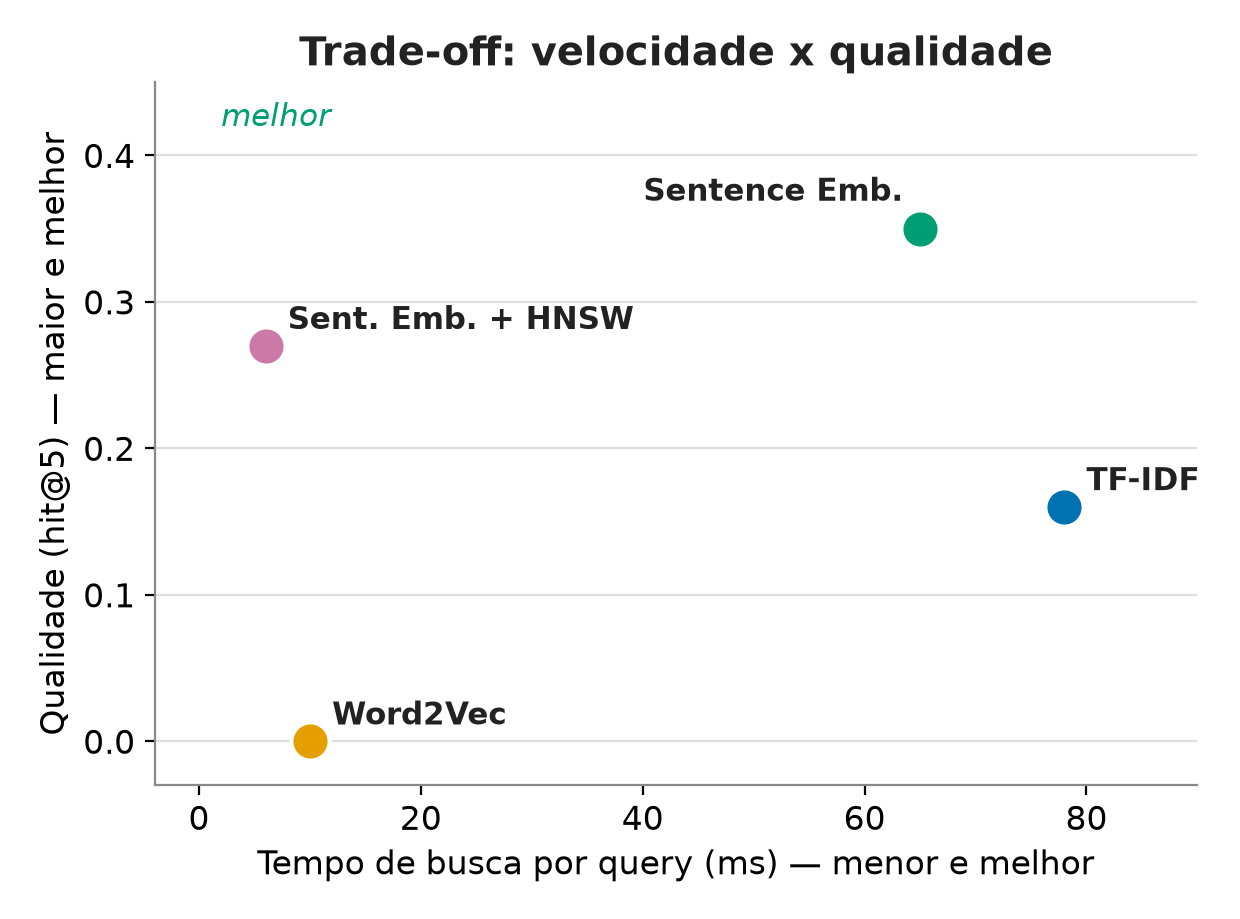
\includegraphics[width=\linewidth]{assets/bench_tradeoff.png}

            \vspace{0.1cm}
            \footnotesize HNSW no canto ideal: quase tão bom quanto a busca exata densa, e muito mais rápido.
        \end{column}
        \begin{column}{0.5\textwidth}
            \centering
            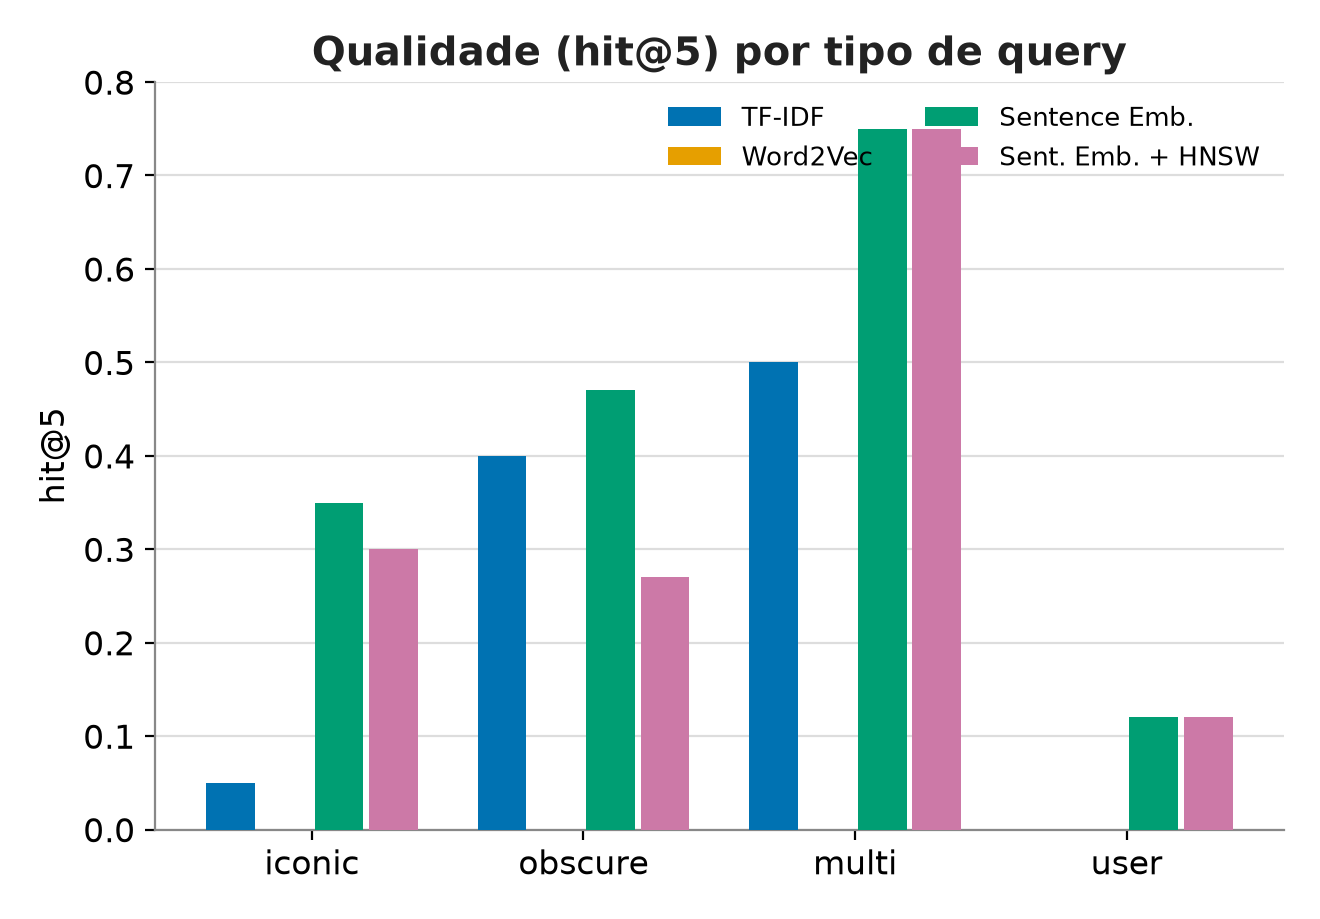
\includegraphics[width=\linewidth]{assets/bench_categoria.png}

            \vspace{0.1cm}
            \footnotesize A semântica (MiniLM) domina; queries de usuário são as mais difíceis; Word2Vec fica zerado.
        \end{column}
    \end{columns}
\end{frame}

% ---------------------------------------------------
% Slide 13: Pontos 11 e 12 - Trade-offs
% ---------------------------------------------------
\begin{frame}{11 e 12. Trade-offs: Qualidade x Tempo}
    \begin{columns}
        \begin{column}{0.5\textwidth}
            \textbf{Tempo de Treino x Qualidade}
            \begin{itemize}
                \item Mais épocas no Word2Vec ou escolha de embeddings mais densos geram vetores melhores, mas aumentam custo de treinamento e memória.
            \end{itemize}
            
            \vspace{0.4cm}
            \textbf{Tempo de Inferência x Qualidade}
            \begin{itemize}
                \item Aumentar o \texttt{top\_k} melhora as chances de recuperar o filme ideal.
                \item Porém, um contexto maior aumenta drasticamente a latência de geração de texto no LLM local.
            \end{itemize}
        \end{column}
        \begin{column}{0.5\textwidth}
            \textbf{Qualidade por tipo de query} \\
            \footnotesize (hit@5, Sentence Embeddings)
            \normalsize
            \begin{itemize}
                \item Queries bem elaboradas: \textbf{0,35--0,47}
                \item Queries de usuário (curtas, vagas): \textbf{0,12}
            \end{itemize}
            \vspace{0.2cm}
            Queries reais são mais difíceis, mas a utilidade \textbf{sobe conforme a semântica melhora}: de 0 (TF-IDF / Word2Vec) para 0,12 (MiniLM). O app ganha alguma utilidade real, ainda que modesta.
            \vspace{0.3cm} \\
            \footnotesize{\textit{Gráfico completo no notebook de análise (Fase 2).}}
        \end{column}
    \end{columns}
\end{frame}

% ---------------------------------------------------
% Slide 14: Ponto 13 - Conclusão
% ---------------------------------------------------
\begin{frame}{13. Demais aspectos relevantes}
    \begin{itemize}
        \item \textbf{Limitações Identificadas:}
        \begin{itemize}
            \item O projeto atua restritamente em inglês.
            \item Mesmo com limitação de temperatura no \textit{prompt}, modelos de linguagem pequenos (Phi-4 Mini) ainda apresentam risco de alucinação e falhas de formatação.
        \end{itemize}
        \vspace{0.4cm}
        \item \textbf{Aprendizados:}
        \begin{itemize}
            \item Compreensão profunda das diferenças práticas (tempo, custo e qualidade) entre buscas exatas e aproximadas.
        \end{itemize}
        \vspace{0.4cm}
        \item \textbf{Próximos Passos:}
        \begin{itemize}
            \item Integração com modelos maiores via nuvem.
            \item Expansão do \textit{dataset} e refinamento do pré-processamento de metadados.
        \end{itemize}
    \end{itemize}
\end{frame}

% ---------------------------------------------------
% Slide 15: Fechamento
% ---------------------------------------------------
\begin{frame}
    \begin{center}
        \Huge \textbf{Obrigado!} \\
        \vspace{1cm}
        \Large Perguntas?
    \end{center}
\end{frame}

\end{document}
